\documentclass[11pt,a4paper,onecolumn,oneside,notitlepage]{article}
\usepackage[utf8]{inputenc}
\usepackage[english]{babel}
\usepackage{csquotes}
\usepackage{amsmath}
\usepackage{amsfonts}
\usepackage{amssymb}
\usepackage{graphicx}
\usepackage{hyperref}
\usepackage{url}
\usepackage[left=2cm,right=2cm,top=2cm,bottom=2cm]{geometry}
\graphicspath{ {./images/} }

\usepackage[backend=biber, %% Hilfsprogramm "biber" (statt "biblatex" oder "bibtex")
	style=authoryear, %% Zitierstil (siehe Dokumentation)
	natbib=true, %% Bereitstellen von natbib-kompatiblen Zitierkommandos
	hyperref=true, %% hyperref-Paket verwenden, um Links zu erstellen
]{biblatex}
\addbibresource{paper.bib}


\author{Manuel Hettich\\

	\begin{small}
		Deep Learning for Natural Language Processing -- SS21 -- Philipp Cimiano and Philipp Heinisch
	\end{small}
}
\title{SemEval-2020 Task 7: Assessing Humor in Edited News Headlines - Subtask 2 (Funnier) with RoBERTa}
\begin{document}
	\maketitle


	\section{Introduction}
	This project is a possible solution to the SemEval-2020 Task 7: Assessing Humor in Edited News Headlines - Subtask 2 (Funnier) with the transformer model RoBERTa \citep{DBLP:journals/corr/abs-1907-11692} using an implementation in Python by Hugging Face \citep{wolf-etal-2020-transformers}.

	The SemEval-2020 Task 7 deals with short humorous edits to news headlines in order to determine if machines can understand which edits are necessary to make a text funny. For this purpose, the authors of this task created new publicly available dataset, called Humicroedit, which contains 15,095 edited news headlines and the humor ratings of five judges per headline \citep{hossain-etal-2019-president}. Most of the edits consist only of replacing a single word, which helps to find the tipping point at which a normal text becomes funny. They were created by crowdsourced editors using original headlines from Reddit and curated by the paper's authors. The judges assigned a numerical rating between 0 - 3 and the ground truth funniness of each data point is the mean of its respective ratings. This grading procedure possibly enables a system to generate multiple edits to a regular text and rank them automatically by their probable funniness. Subtask 2 of SemEval-2020 Task 7 concerns the prediction of the funnier of two edited headlines. We are given the original headline as well as two edited versions of the same headline to predict the funnier version of the two by using the classification accuracy as evaluation metric.

	This task is a good first step to better understand what makes a regular text become funny by editing and possibly enable machines to create them automatically, rate jokes from professional comedians and personalize funny headlines to individual readers. The data also connects with classic theories of humor, such as incongruity, superiority and setup/punchline. The authors argue that computerized humor generation has not seen much progress while automatic humor recognition made some good advances over the last few years. They claim this is not surprising since the same principle applies to humans: they can easily recognize something funny but often fail to produce funny content themselves due to the complex nature of what humor entails (in-depth world-knowledge, common sense and relationships of objects acress different layers of understanding). This challenge is further increased by the shortness of news headlines and the small edits employed in this task.

	In this paper, a possible solution to the given task is demonstrated with the pretrained language model (PLM) RoBERTa, which is based on Google's BERT model and was released in 2019. At first, related work is described by taking a closer look at another published solution to the task which differs from my own. Afterwards, the model I have used and the corresponding architecture as well as my chosen language model are introduced in more detail. Finally, my test results are compared to the related work and some conclusions are discussed in order to possibly improve my approach in the future.


	\section{Related work}
	The team UniTuebingenCL (Charlotte Sophie Ammer, Lea Hannah Grüner) submitted their work for both sub-tasks of the shared task 7 at the 14th International Workshop on Semantic Evaluations in 2020 \citep{ammer-gruner-2020-unituebingencl}. They employed a ridge regression model using Elmo and Glove embeddings as well as Truncated Singular Value Decomposition. The original and edited versions of each headline were encoded using Tf-Idf weighting and they took the edit distance between the two different embeddings into account. In addition, they also used a long short term memory model recurrent network (LSTM) with the Keras library in a twin architecture to process the different headline versions simultaneously resulting in a merged output. In terms of pre-processing, the authors removed non-alphanumeric characters, turned all characters into lower-case and encoded sentences as n-grams by using their Tf-Idf weights. Also the sentences were padded to achieve uniform lengths for the LSTM approach.

	In order to solve subtask 2, the authors used the same ridge regression they used in sub-task 1 with the same parameters. The predictions of the model for each of the two headline versions were compared to determine the funnier version as the result for this sub-task. The ridge regression model for sub-task 1 used a normalization of the output to limit the predictions at a value between zero and three and their parameters were tuned using a grid search.

	The author's approach landed them at positions 18/48 for sub-task 1 and 14/31 for sub-task 2 with an accuracy value of 0.6183 in the competition. They notice the advantage of their ridge regression model with Glove 100d embeddings for sub-task 1 over their alternative twin LSTM approach and also received a better ranking with their linear model in the evaluation phase. The authors describe the challenges of both sub-tasks and conclude that a mixture of fine-tuning and pretrained embeddings yielded the best results and that their experimenting with different parameters and features did not result in better predictions for subtask 2. Finally, they claim the threshold of 0.5 RMSE score for sub-task 1 was surpassed by only few of the competitors and the tasks seemed challenging for most participants.


	\section{Method}
	For this project I have chosen to use the RoBERTa model, which was proposed by Liu et al. in 2019 \citep{DBLP:journals/corr/abs-1907-11692} and it is based on Google's BERT model released in 2018. I am using the Python implementation by Hugging Face \citep{wolf-etal-2020-transformers} and I selected this model because it demonstrated the best test results in previous benchmarks for the same task \citep{DBLP:journals/corr/abs-2008-00304}, achieving a similar accuracy to the fourth best team in the SemEval-2020 competition.

	The RoBERTa model has modified hyperparameters, removed the next-sentence pretraining objective from the original BERT model and it was trained on larger mini-batches and learning rates as well as on longer sequences and the masking pattern applied to the training data was changed dynamically. The authors of RoBERTa state that according to their research the BERT model was "significantly undertrained" and that their improvements can "match or exceed the performance of every mode published after it" \citep{DBLP:journals/corr/abs-1907-11692}. They achieved similar results to other state-of-the-art models in different NLP benchmark datasets like GLUE, RACE and SQuAD. Interestingly, RoBERTa was also trained on the CC-News corpus, which contains over 60 million English news articles and it might explain some of RoBERTa's advantages over other approaches for the news headlines data in this task.

	In general, transformer models like RoBERTa are deep learning models based on neural networks which employ the concept of attention by putting different weights on different parts of the input \citep{DBLP:journals/corr/VaswaniSPUJGKP17}. Besides natural language processing (NLP), they are also used in computer vision programs and they have reduced training times due to parallelization compared to recurrent neural networks (RNNs) which process input data in order. Instead, transformers identify the context of each word in the sentence and thereby unmask their meaning. This approach enables researchers to use parallelization, since different parts of the input data can be processed at the same time and nowadays, transformers have become the preferred model for NLP tasks \citep{wolf-etal-2020-transformers}.

	In order to tokenize each data entry in the Humicroedit dataset, I am pre-processing it by generating two sentences per entry, one with the original word and one with the edited word included. Both sentences are stringed together and tokenized as a pair of sequences using the pre-trained RoBERTa tokenizer by HuggingFace (class transformers.RobertaTokenizer, version "roberta-base"). A pair of sequences "A" and "B" are concatenated using the language model's special tokens in the following way: \verb|<s> A </s></s> B </s>|. Afterwards, the sequence pairs are encoded into input IDs which are used for training the model or calculating its prediction for the resulting label (see figure \ref{fig1}).

	\begin{figure}
		\begin{center}
			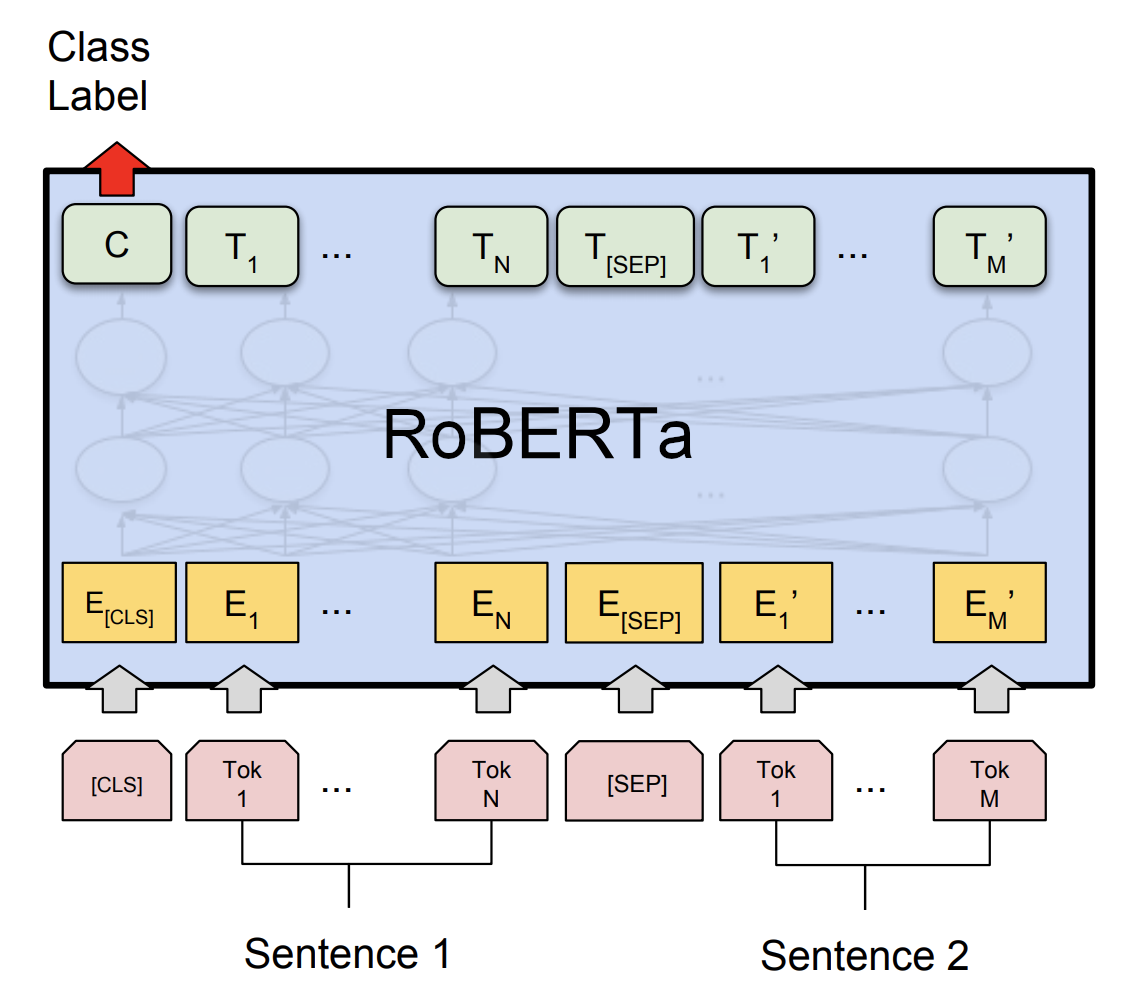
\includegraphics[width=0.4\linewidth]{images/roberta_sequence.png}
		\end{center}
		\caption{RoBERTa processing a sequence pair as input with special tokens displayed.}\label{fig1}
	\end{figure}

	For training the language model, I am using a similar approach to the author's of UniTuebingenCL \citep{ammer-gruner-2020-unituebingencl} in that I am training it first on the Humicroedit dataset for subtask 1 with a RMSE metric for 10 epochs and then use it as a single-shot inference for predicting a grade for both versions of a news headline in the test dataset for subtask 2. Finally, both predictions for a data entry are compared and the higher score determines which version is predicted as being the funnier one. The accuracy metric is used to determine how well the model has been trained for this task. The model itself is a specific version of RoBERTa, which is especially well suited for sequence classification / regression tasks like this one. It contains a linear layer on top of the final pooled output with 768 hidden states, 12 attention heads and 12 layers.


	\section{Evaluation}
	My final final test runs result in an accuracy value of 0.4533 for subtask 2, which is significantly worse than the model UniTuebingenCL \citep{ammer-gruner-2020-unituebingencl} with an accuracy of 0.618 for the same task. In the official competition this result would have placed me at ranking 29/32 according to the published results and benchmarks (see figure \ref{fig2}).

	It is also interesting to note that most predictions of my fine-tuned language model are very similar with a predicted funniness grade at around 1.0 per comparison of original vs. edited headline as a sequence pair. This result is similar to the author's findings of the original dataset \citep{hossain-etal-2019-president}.

	\begin{figure}
		\begin{center}
			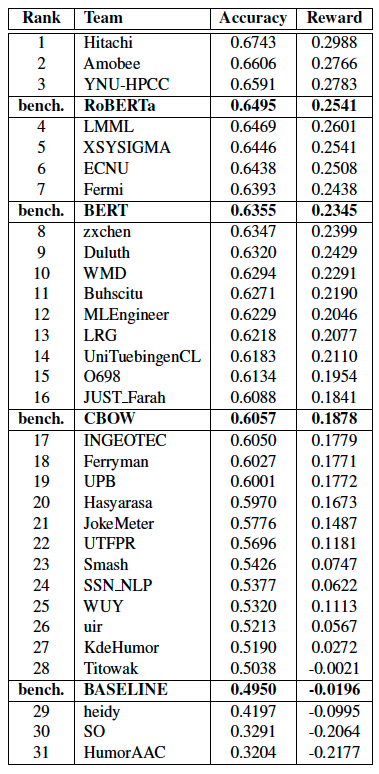
\includegraphics[width=0.3\linewidth]{images/paper_benchmarks.png}
		\end{center}

		\caption{Official results and benchmarks for Subtask 2.}\label{fig2}
	\end{figure}

	Additionally, fine-tuning the language model took a very long time and I was only able to shorten this process by a certain factor by using Google's Colab features. However, limited computational resources in the free tier of their service restricted me in my efforts to benchmark different hyperparameter settings and only allowed me to run few training rounds.


	\section{Conclusion}
	Due to limited computational resource without a GPU, I am unfortunately unable to train my chosen language model for a significant amount of time on my personal computer hardware, which resulted in rather poor results in my test runs. It would be interesting to see if a longer training duration or an extended search for better hyperparameter settings would result in significantly improvements of my test results.

	In general, I believe RoBERTa and other BERT-based language models are well-suited for this kind of classification task and further improvements in the pre-training strategies are destined to result in better outcomes for everyone without the need for significant computational resources.

	\printbibliography
\end{document}